\documentclass[10pt]{article}

% ---------------------------------------------------------------- page & fonts
\usepackage[a4paper,top=0.6in,bottom=0.55in,left=0.75in,right=0.75in]{geometry}
\usepackage[T1]{fontenc}
\usepackage[default]{sourceserifpro}
\usepackage{sourcesanspro}
\usepackage{amsmath,amssymb}
\usepackage[italic,defaultmathsizes]{mathastext}
\usepackage{microtype}

% ---------------------------------------------------------------- layout tools
\usepackage{xcolor}
\usepackage{booktabs}
\usepackage{array}
\usepackage{colortbl}
\usepackage{enumitem}
\usepackage{titlesec}
\usepackage{ragged2e}
\usepackage{tikz}
\usepackage[most]{tcolorbox}
\usepackage{fontawesome5}
\usepackage[hidelinks]{hyperref}
\usetikzlibrary{positioning,calc,arrows.meta}

% ---------------------------------------------------------------- palette (Okabe--Ito accents)
\definecolor{ink}{HTML}{1B1F24}
\definecolor{slate}{HTML}{56626E}
\definecolor{accent}{HTML}{0072B2}
\definecolor{go}{HTML}{009E73}
\definecolor{stop}{HTML}{D55E00}
\definecolor{warn}{HTML}{B07A00}
\definecolor{wash}{HTML}{EDF4F9}
\definecolor{hair}{HTML}{D3DCE4}

\color{ink}
\arrayrulecolor{hair}

% ---------------------------------------------------------------- section style
\titleformat{\section}
  {\normalsize\sffamily\bfseries\color{ink}}
  {\raisebox{-0.5pt}{\tikz\node[fill=accent,text=white,rounded corners=1.5pt,
     inner xsep=4pt,inner ysep=1.2pt,font=\sffamily\bfseries\footnotesize]{\thesection};}}
  {0.6em}{}[\vspace{-0.45em}{\color{hair}\rule{\linewidth}{0.6pt}}]
\titlespacing*{\section}{0pt}{0.85em}{0.4em}

\setlist{nosep,leftmargin=1.3em}
\setlist[itemize]{label=\textcolor{accent}{\scriptsize\faSquare}}
\newlist{tasks}{itemize}{1}
\setlist[tasks]{label=\textcolor{slate}{\faSquare[regular]},leftmargin=1.5em,nosep}

\setlength{\parskip}{0.3em}
\setlength{\parindent}{0pt}
\renewcommand{\arraystretch}{1.05}

% ---------------------------------------------------------------- helpers
\newcolumntype{L}[1]{>{\RaggedRight\arraybackslash}p{#1}}
\newcommand{\lead}[1]{{\sffamily\bfseries #1}}
\newcommand{\badge}[2]{%
  \tikz[baseline=(b.base)]{\node[fill=#1!12,text=#1!80!black,rounded corners=2pt,
    inner xsep=3.5pt,inner ysep=1.3pt,font=\sffamily\bfseries\scriptsize] (b) {#2};}}

\newtcolorbox{stagecard}[2][]{
  enhanced, breakable, colback=white, colframe=hair, boxrule=0.6pt, arc=2pt,
  left=7pt, right=7pt, top=4pt, bottom=4pt,
  fonttitle=\sffamily\bfseries\footnotesize, coltitle=ink, colbacktitle=wash,
  title={#2}, #1}

\newcommand{\flag}[2]{\colorbox{#1!12}{\textcolor{#1!80!black}{\sffamily\bfseries\tiny #2}}}
\newcommand{\cardtag}[1]{{\sffamily\scriptsize\color{slate} #1}}

\newtcolorbox{keybox}[1][]{
  enhanced, breakable, colback=wash, colframe=accent, boxrule=0pt,
  leftrule=2.5pt, arc=1.5pt, left=7pt, right=7pt, top=4pt, bottom=4pt, #1}

% ---------------------------------------------------------------- OPTIONAL: domain schematic
% Project-specific. Delete and write your own picture macro for your system.
\newcommand{\netpanel}[2]{%
  \begin{scope}
    \draw[rounded corners=3pt,fill=wash,draw=hair,line width=0.5pt]
      (-0.34,-0.34) rectangle (2.14,2.14);
    \foreach \i/\x/\y in {1/0/0,2/0.9/0,3/1.8/0,4/0/0.9,5/0.9/0.9,6/1.8/0.9,
                          7/0/1.8,8/0.9/1.8,9/1.8/1.8}
      {\coordinate (n\i) at (\x,\y);}
    \foreach \a/\b/\w in {#2} {\draw[line width=\w pt,slate,line cap=round] (n\a)--(n\b);}
    \foreach \i in {1,...,9} {\fill[ink] (n\i) circle (1.5pt);}
    \node[font=\sffamily\bfseries\scriptsize,color=ink] at (0.9,-0.62) {#1};
  \end{scope}}

\begin{document}
\pagestyle{empty}

% ================================================================= MASTHEAD
% The one-line question, then the subtitle, then the provenance line.
\begin{tcolorbox}[enhanced,colback=accent,colframe=accent,boxrule=0pt,arc=2pt,
  left=10pt,right=10pt,top=7pt,bottom=7pt]
  {\sffamily\bfseries\large\color{white} [THE QUESTION, AS A QUESTION]}\\[1pt]
  {\sffamily\color{white!88} [one-line expansion]
   \quad$\cdot$\quad action brief}\\[3pt]
  {\sffamily\scriptsize\color{white!80} YYYY-MM-DD \quad$\cdot$\quad short form of
   [the long document] \quad$\cdot$\quad draft for team decision}
\end{tcolorbox}

\vspace{0.45em}

% ================================================================= TL;DR
% Left: the idea in one paragraph. Right: what you need from the reader.
% Keep the right column to things only they can give you.
\begin{tcolorbox}[enhanced,colback=wash,colframe=accent,boxrule=0pt,leftrule=2.5pt,
  arc=1.5pt,left=8pt,right=8pt,top=5pt,bottom=5pt]
\begin{minipage}[t]{0.49\linewidth}\vspace{0pt}
\lead{TL;DR \;·\; the idea.} [Two competing explanations. Nobody has separated
them. Here is the control that separates them. Either answer is a paper.]
\end{minipage}\hfill
\begin{minipage}[t]{0.012\linewidth}\vspace{0pt}%
{\color{accent!30}\rule{0.6pt}{2.9cm}}\end{minipage}\hfill
\begin{minipage}[t]{0.45\linewidth}\vspace{0pt}
\lead{Input:}
\begin{itemize}[leftmargin=1.1em]
\item [data / files / configurations only they have]
\item [a judgement call only they can make]
\item [the part of the plan you want them to read]
\end{itemize}
\vspace{0.25em}
Building, running, and analysis sit on our side.
\end{minipage}
\end{tcolorbox}

% ================================================================= SECTIONS
\section{The question}

[Both candidate mechanisms, stated fairly, one paragraph each. The reader must
believe you would be happy with either answer.]

\begin{keybox}
\lead{Falsifiable core:} [the single sentence that can come out false.]
\end{keybox}

\section{The experiment}

[The arms. What is held fixed, what is varied, and why that isolates the
mechanism.]

\lead{Primary observable:} [one quantity, defined precisely.]

\lead{Primary endpoint:} [the paired comparison you will actually test.]

\lead{Hard gate before any comparison:} [the confound audit that must pass
first.]

\section{Plan}

% --- stage flow figure -------------------------------------------------
% One node per stage, left to right, with the exit conditions hanging off
% the right-hand side. Keeps the reader oriented before the cards below.
\begin{center}
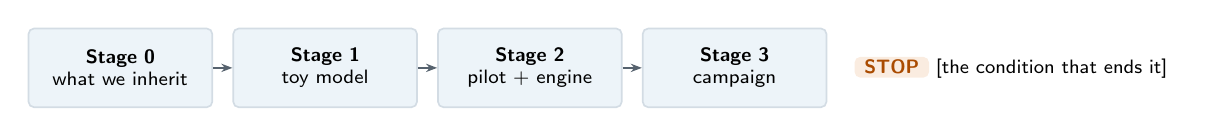
\begin{tikzpicture}[
  stage/.style={draw=hair,fill=wash,rounded corners=2pt,line width=0.6pt,
    font=\sffamily\scriptsize,align=center,minimum height=1.0cm,text width=2.1cm},
  gate/.style={font=\sffamily\scriptsize,align=left,text width=4.2cm,anchor=west},
  flow/.style={-{Stealth[length=4pt]},draw=slate,line width=0.6pt}]
  \node[stage] (s0) at (0,0)   {\textbf{Stage 0}\\what we inherit};
  \node[stage] (s1) at (2.6,0) {\textbf{Stage 1}\\toy model};
  \node[stage] (s2) at (5.2,0) {\textbf{Stage 2}\\pilot + engine};
  \node[stage] (s3) at (7.8,0) {\textbf{Stage 3}\\campaign};
  \foreach \a/\b in {s0/s1,s1/s2,s2/s3} {\draw[flow] (\a)--(\b);}
  \node[gate] at (9.2,0) {\badge{stop}{STOP} [the condition that ends it]};
\end{tikzpicture}
\end{center}

% --- one card per stage ------------------------------------------------
% Each card answers three things: the question this stage settles, what it
% hands the next stage, and how it can end the project.
\begin{stagecard}{Stage 0 \;·\; [what this stage decides]}
\cardtag{Question it answers.} [...]

\cardtag{Hands on.} [the object the next stage consumes]

\cardtag{Can end the project if.} [...] \flag{stop}{STOP RISK}

\begin{tasks}
\item [task]
\item [task]
\end{tasks}
\end{stagecard}

\vspace{0.4em}

\begin{stagecard}{Stage 1 \;·\; [what this stage decides]}
\cardtag{Question it answers.} [...]
\end{stagecard}

\section{Explicitly dropped}

% Say what you are NOT doing, before a reader asks. This is the section that
% buys trust.
\begin{itemize}
\item [thing not done, and the one-line reason]
\end{itemize}

\section{Decisions}

\begin{itemize}
\item \badge{go}{G1} [gate that lets the work continue]
\item \badge{stop}{G2} [gate that stops it]
\item \badge{accent}{GUARD} [a question deliberately held separate]
\end{itemize}

\section{What we need from the team}

\begin{enumerate}[label=\textcolor{accent}{\sffamily\bfseries\footnotesize\arabic*.},leftmargin=1.6em]
\item [the blocking item] \badge{stop}{BLOCKING} and the first thing to ask about.
\item [a go / no-go call]
\end{enumerate}

\vspace{0.1em}
{\color{hair}\rule{\linewidth}{0.6pt}}\\[0.2em]
{\sffamily\scriptsize\color{slate} Full statistical design, prior-art
confrontation, figure plan, and risk register are in [the long document].}

\end{document}
